\documentclass{beamer}
 
\usepackage[utf8]{inputenc}
 \usefonttheme{structuresmallcapsserif}
\usepackage{listings}
\newsavebox{\mybox}

%\lstdefinestyle{myCustomMatlabStyle}{
%  language=Matlab,
%  numbers=left,
%  stepnumber=1,
%  numbersep=10pt,
%  tabsize=4,
%  showspaces=false,
%  showstringspaces=false
%}
% 
 
%Information to be included in the title page:
\title{Linear Elasticity Problem in 3D }
\author{Guhan}
\date{Jan. 11, 2018}
 
 
 
\begin{document}
 
\frame{\titlepage}
 
\begin{frame}
\frametitle{Objective}
\begin{itemize}
		\vfill
		\item{Solve linear elasticity equation for a test problem using FEniCS}
		\vfill
		\item{Compare the result against analytical solution}
		\vfill
		\item{Perform convergence study}
		\vfill
		\item{Idea is to use this result as a benchmark/validation case for any new codes and methods that we may develop in future}
		\vfill
\end{itemize}
\end{frame}
 
 \begin{frame}
\frametitle{Installing FEniCS}
\begin{itemize}
		\vfill
		\item{Installed FEniCS using Docker}
		\vfill
		\item{Docker allows for identical deployment across your laptop, the cloud or  any high performance computing environments}
		\vfill
		\item{Using Macbook for the project}
		\vfill
		\item{Visualizing solutions and post processing using Paraview}
		\vfill
\end{itemize}
\end{frame}


 \begin{frame}
\frametitle{Problem Description}
\begin{itemize}
		\vfill
		\item{Cantilever beam in 3D, fixed at left end with a edge (surface) load at the right end}
		\vfill
		\item{Load =1, Stifness=1, Poisson ratio=0.3}
		\vfill
		\item{Use 3D Brick elements with midnodes (quadratic interpolation in each direction)}
		\vfill
\begin{figure}
\includegraphics[width=.9\textwidth]{fea_0}
\end{figure}
\end{itemize}
\end{frame}

 \begin{frame}
\frametitle{Step 1: Running example problem from FEniCS tutorial}
\begin{itemize}
		\vfill
		\item{Example can be found in section 3.3.3 (page 52) of the tutorial}
		\vfill
		\item{It is basically modeling a clamped beam deformed under its own weight in 3D}
		\vfill
		\item{The code and the results are attached in the next couple of slides}
		\vfill
\end{itemize}
\end{frame}


 \begin{frame}[fragile, allowframebreaks]
\frametitle{Code from the tutorial - Cantilever beam in 3D under its own weight}
\begin{lstlisting}[language=Python, basicstyle=\ttfamily\tiny,  keywordstyle=\color{blue},  numbers=left,  stepnumber=1, numbersep=10pt, tabsize=4, showspaces=false, showstringspaces=false]
from __future__ import print_function
from fenics import *
# Scaled variables
L = 1; W = 0.2
mu = 1
rho = 1
delta = W/L
gamma = 0.4*delta**2
beta = 1.25
lambda_ = beta
g = gamma

# Create mesh and define function space
mesh = BoxMesh(Point(0, 0, 0), Point(L, W, W), 10, 3, 3)
V = VectorFunctionSpace(mesh, 'P', 1)

# Define boundary condition
tol = 1E-14

def clamped_boundary(x, on_boundary):
    return on_boundary and x[0] < tol

bc = DirichletBC(V, Constant((0, 0, 0)), clamped_boundary)

# Define strain and stress

def epsilon(u):
    return 0.5*(nabla_grad(u) + nabla_grad(u).T)
    #return sym(nabla_grad(u))

def sigma(u):
    return lambda_*nabla_div(u)*Identity(d) + 2*mu*epsilon(u)

# Define variational problem
u = TrialFunction(V)
d = u.geometric_dimension()  # space dimension
v = TestFunction(V)
f = Constant((0, 0, -rho*g))
T = Constant((0, 0, 0))
a = inner(sigma(u), epsilon(v))*dx
L = dot(f, v)*dx + dot(T, v)*ds

# Compute solution
u = Function(V)
solve(a == L, u, bc)

# Plot solution
plot(u, title='Displacement', mode='displacement')

# Plot stress
s = sigma(u) - (1./3)*tr(sigma(u))*Identity(d)  # deviatoric stress
von_Mises = sqrt(3./2*inner(s, s))
V = FunctionSpace(mesh, 'P', 1)
von_Mises = project(von_Mises, V)
plot(von_Mises, title='Stress intensity')

# Compute magnitude of displacement
u_magnitude = sqrt(dot(u, u))
u_magnitude = project(u_magnitude, V)
plot(u_magnitude, 'Displacement magnitude')
print('min/max u:',
      u_magnitude.vector().array().min(),
      u_magnitude.vector().array().max())

# Save solution to file in VTK format
File('elasticity/displacement.pvd') << u
File('elasticity/von_mises.pvd') << von_Mises
File('elasticity/magnitude.pvd') << u_magnitude

\end{lstlisting}
\end{frame}

 \begin{frame}
\frametitle{Sample result}
\begin{figure}
\centering
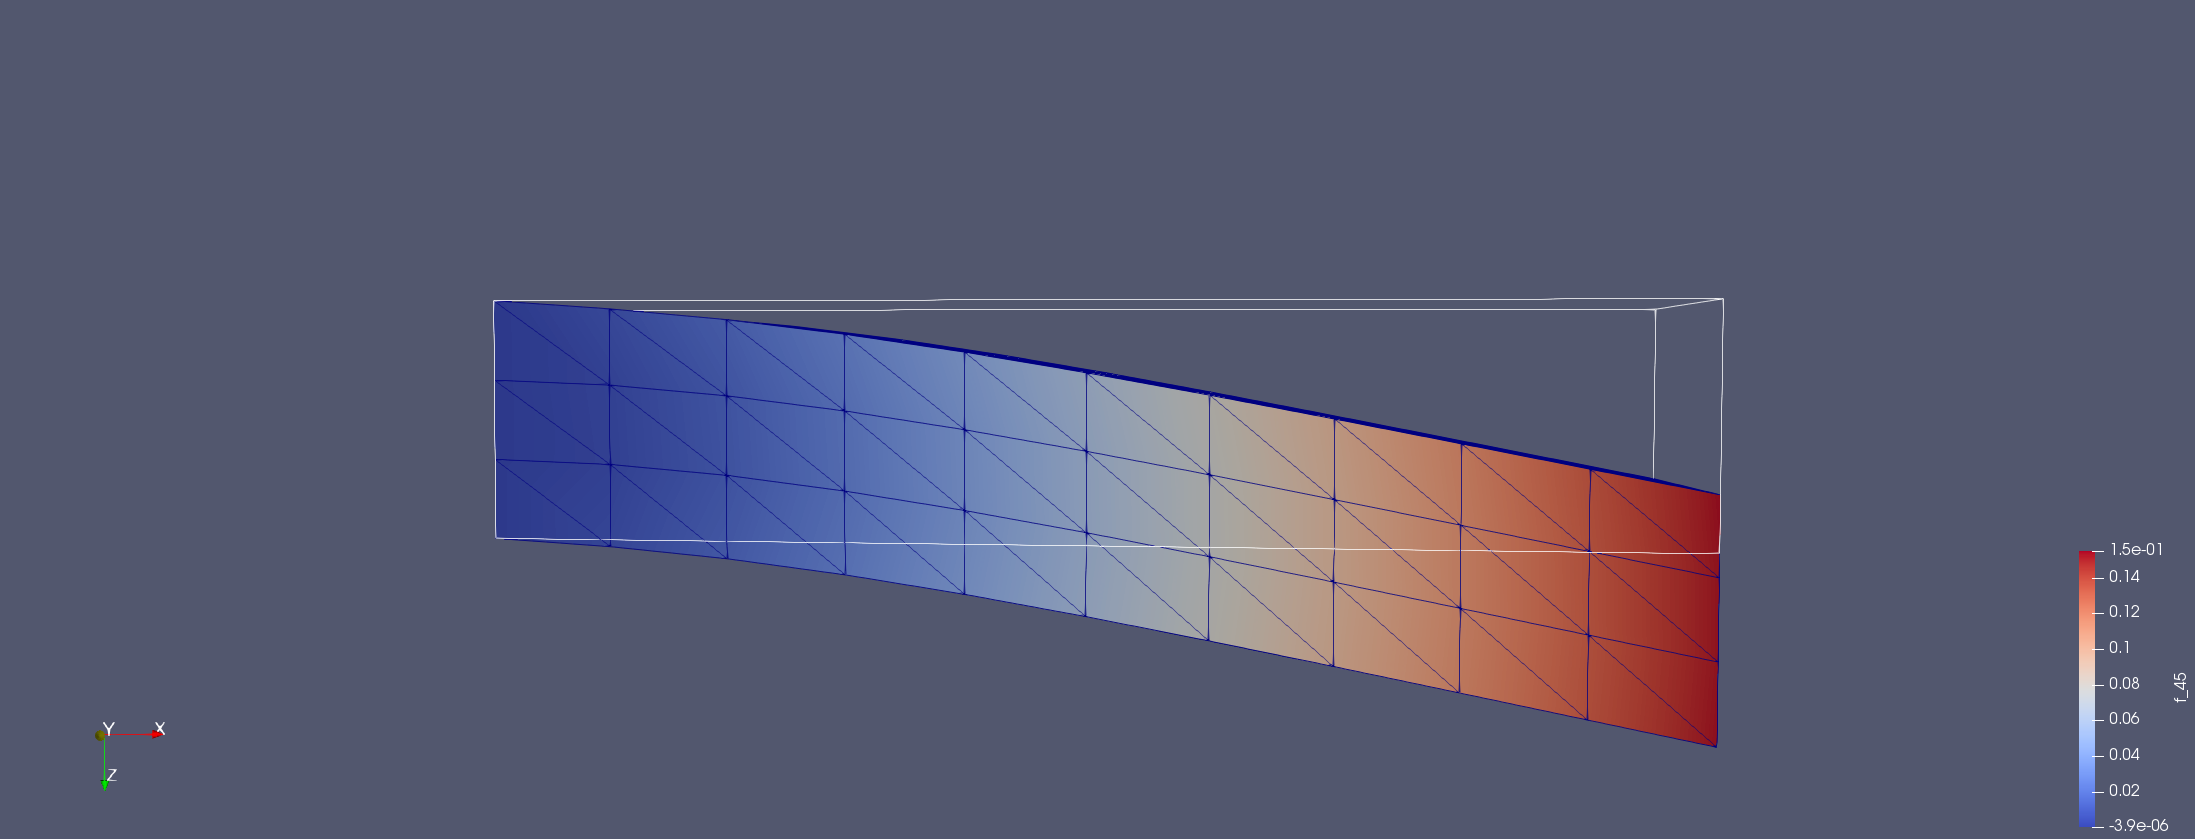
\includegraphics[width=1\textwidth]{Beam3DFigure}
\end{figure}
\end{frame}


 \begin{frame}
\frametitle{Step 2: Modifying the example problem - Adding Point/Surface load}
\begin{itemize}
		\vfill
		\item{The idea here is to modify the code to suit our problem where a surface load is applied at the end, instead of deforming under its own weight. This would be the first step.}
		\vfill
		\item{Once this is successful, then we can go ahead and modify the problem more to include properties like stiffness, poisson ratio and changing the finite element type like using brick element etc.}
		\vfill
\end{itemize}
\end{frame}

 \begin{frame}[fragile]
\frametitle{Step 2.1: Removing body force and adding traction in the code}
\begin{itemize}
		\vfill
		\item{Body force is removed}
		\begin{lstlisting}[language=Python, basicstyle=\ttfamily\small,  keywordstyle=\color{blue}]
	f = Constant((0, 0, 0))
		
\end{lstlisting}
\end{itemize}

\begin{itemize}
		\vfill
		\item{Defining traction: arbitrarily choosing -10 as the value here.}
		\begin{lstlisting}[language=Python, basicstyle=\ttfamily\small,  keywordstyle=\color{blue}]
	T = Constant((0, 0, -10))
		
\end{lstlisting}
	
		\vfill
\end{itemize}
\end{frame}

 \begin{frame}[fragile]
\frametitle{ Step 2.2: Defining the boundaries}
\begin{itemize}
		\vfill
		\item{A subdomain is defined over which load is applied and integrated later}
		\vfill
		\item{Here subdomain is constructed by way of using instance of the subdomain class}
		\begin{lstlisting}[language=Python, basicstyle=\ttfamily\small,  keywordstyle=\color{blue}]
class Right(SubDomain):
def inside(self, x, on_boundary):
 return near(x[0], L)

\end{lstlisting}

		\vfill
		\item{If a point is in the region x=L, the it is identified as the right side. Similar instance is used for the left side}
				\begin{lstlisting}[language=Python, basicstyle=\ttfamily\small,  keywordstyle=\color{blue}]
class Left(SubDomain):
def inside(self, x, on_boundary):
return near(x[0], 0.0)
\end{lstlisting}
		\vfill
		\item{Initializing sub-domain instances}
		\begin{lstlisting}[language=Python, basicstyle=\ttfamily\small,  keywordstyle=\color{blue}]
left = Left()
right = Right()

\end{lstlisting}
		
\end{itemize}
\end{frame}

 \begin{frame}[fragile]
\frametitle{ Step 2.3: Defining Meshfunction and marking the mesh}
\begin{itemize}
		\vfill
		\item{Defining MeshFunction for the boundary domains - not very confident about this part}
		\begin{lstlisting}[language=Python, basicstyle=\ttfamily\small,  keywordstyle=\color{blue}]
sub_domains = MeshFunction("size_t", mesh)

\end{lstlisting}
		\vfill
		\item{All the values of MeshFunction is initially set to 0 and then left and right instances are used to mark the regions as 2 and 1 respectively}
		\begin{lstlisting}[language=Python, basicstyle=\ttfamily\small,  keywordstyle=\color{blue}]
sub_domains.set_all(0)
right.mark(sub_domains, 1)
left.mark(sub_domains, 2)

\end{lstlisting}	

\end{itemize}
\end{frame}



 \begin{frame}[fragile]
\frametitle{ Step 2.4: Applying the load over the right end boundary}
\begin{itemize}
	         \vfill
	         \item{Defining measures associated with the boundaries. Integration over subregions can be specified by measures with different integer labels as arguments}
	         		\begin{lstlisting}[language=Python, basicstyle=\ttfamily\small,  keywordstyle=\color{blue}]
ds = Measure("ds")[sub_domains]
\end{lstlisting}	
		\vfill
		\item{Define the variational form using the measures developed. The load or traction is integrated only over the right end subdomain previously marked as 1}	
		\begin{lstlisting}[language=Python, basicstyle=\ttfamily\small,  keywordstyle=\color{blue}]
T = Constant((0, 0, -10))
a = inner(sigma(u), epsilon(v))*dx
L = dot(T, v)*ds(1)
\end{lstlisting}	
\end{itemize}


\end{frame}
 \begin{frame}[fragile, allowframebreaks]
\frametitle{Complete code - Cantilever beam in 3d with face load at right end}
\begin{lstlisting}[language=Python, basicstyle=\ttfamily\tiny,  keywordstyle=\color{blue},  numbers=left,  stepnumber=1, numbersep=10pt, tabsize=4, showspaces=false, showstringspaces=false]

from __future__ import print_function
from fenics import *

# Scaled variables
L = 1; W = 0.2
mu = 1
rho = 1
delta = W/L
gamma = 0.4*delta**2
beta = 1.25
lambda_ = beta
g = gamma

# Create mesh and define function space
mesh = BoxMesh(Point(0, 0, 0), Point(L, W, W), 10, 3, 3)
V = VectorFunctionSpace(mesh, 'P', 1)

# Define boundary condition

class Left(SubDomain):
    def inside(self, x, on_boundary):
      return near(x[0], 0.0)
    
class Right(SubDomain):
    def inside(self, x, on_boundary):
#return on_boundary and  abs(x[0]-L) < 0.2 and abs(x[1]-W) < 0.2  and abs(x[1]-W) < 0.2
      return near(x[0], L)
      
left = Left()
right = Right()
sub_domains = MeshFunction("size_t", mesh)
sub_domains.set_all(0)
right.mark(sub_domains, 1)
left.mark(sub_domains, 2)

bc = DirichletBC(V, Constant((0, 0, 0)), left)
ds = Measure("ds")[sub_domains]
#ds = ds(subdomain_data = MeshFunction)

# Define strain and stress

def epsilon(u):
    return 0.5*(nabla_grad(u) + nabla_grad(u).T)
    #return sym(nabla_grad(u))

def sigma(u):
    return lambda_*nabla_div(u)*Identity(d) + 2*mu*epsilon(u)

# Define variational problem
u = TrialFunction(V)
d = u.geometric_dimension()  # space dimension
v = TestFunction(V)
f = Constant((0, 0, 0))

#Load at the right end
T = Constant((0, 0, -10))
a = inner(sigma(u), epsilon(v))*dx
L = dot(T, v)*ds(1)

# Compute solution
u = Function(V)
solve(a == L, u, bc)

# Plot solution
plot(u, title='Displacement', mode='displacement')

# Plot stress
s = sigma(u) - (1./3)*tr(sigma(u))*Identity(d)  # deviatoric stress
von_Mises = sqrt(3./2*inner(s, s))
V = FunctionSpace(mesh, 'P', 1)
von_Mises = project(von_Mises, V)
plot(von_Mises, title='Stress intensity')

# Compute magnitude of displacement
u_magnitude = sqrt(dot(u, u))
u_magnitude = project(u_magnitude, V)
plot(u_magnitude, 'Displacement magnitude')
print('min/max u:',
      u_magnitude.vector().array().min(),
      u_magnitude.vector().array().max())

# Save solution to file in VTK format
# File('elasticity/displacement.pvd') << u
# File('elasticity/von_mises.pvd') << von_Mises
# File('elasticity/magnitude.pvd') << u_magnitude

\end{lstlisting}
\end{frame}

 \begin{frame}[fragile]
\frametitle{Possible reasons for code failing}
\begin{itemize}
		\vfill
		\item{I am getting segmentation error right now - have to install Valgrind to find any memory leakage}
		\vfill
		\item{I am also not confident about the way subdomains and meshfunctions are defined - I am still working on it. I am not sure by setting subdomains at x=0 and x=L, it means the entire face or just the edge. This is where I am digging deep now}
		\vfill
		\item{I am not yet clear how the subdomains are integrated into the solver}
		\vfill
\end{itemize}
\end{frame}

 \begin{frame}
\frametitle{Other ways to make it work}
\begin{itemize}
		\vfill
		\item{One way is to use a third party meshing tool (like Gmsh) and import the meshed geometry into FEniCS}
		\vfill
		\item{There are couple of other ways that I found in FEniCS forum - yet to try them all. Will update this space as I learn more}
		\vfill
\end{itemize}
\end{frame}

 \begin{frame}[fragile]
\frametitle{Update - Jan 20: Visualizing Meshes}
\begin{itemize}
		\vfill
		\item{I wanted to make sure the boundaries are captured right by visualizing them - made following changes in code}
	\begin{lstlisting}[language=Python, basicstyle=\ttfamily\small,  keywordstyle=\color{blue}]
sub_domains = FacetFunction("size_t", mesh)
sub_domains.set_all(0)	
left.mark(sub_domains, 10)
right.mark(sub_domains,10)

\end{lstlisting}
\vfill
\item{The values are set to 10 just for visualization purpose. Red means 10 and Blue means 0}

\begin{figure}
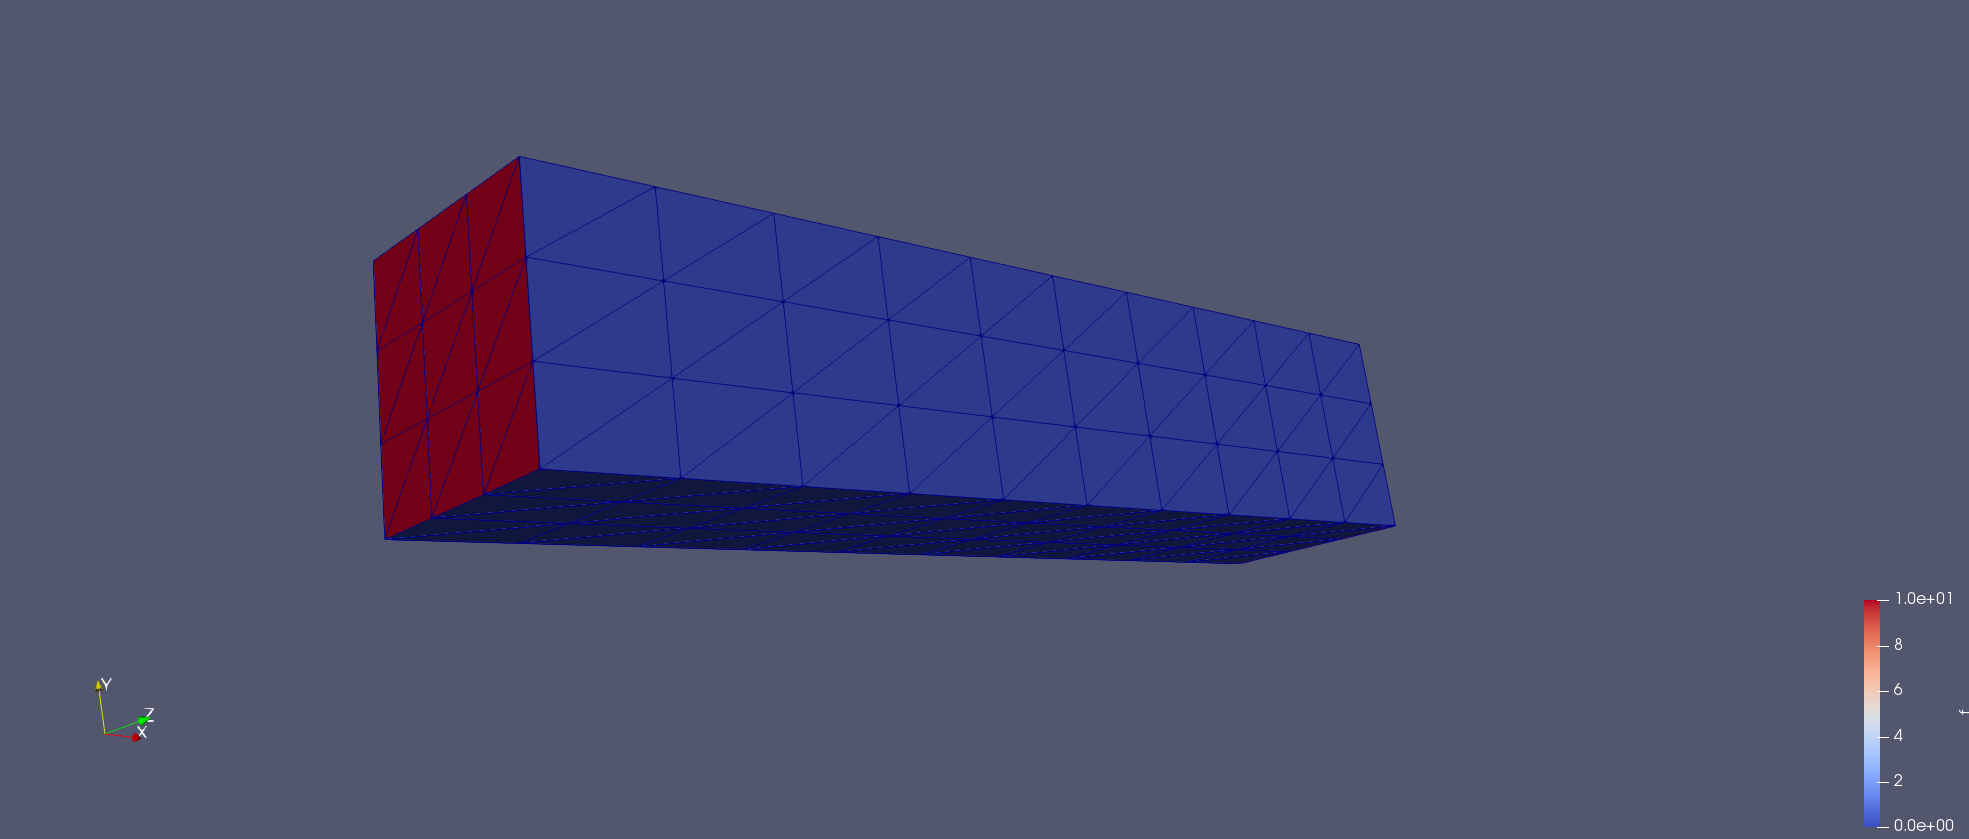
\includegraphics[width=0.7\textwidth]{Fixed_End}
\end{figure}
\vfill
\item{Here we see the fixed end at x=0 marked in red. Similarly at x=L, the right end is identified and marked in red.}

\end{itemize}
\end{frame}

 \begin{frame}[fragile]
 \frametitle{Update - Jan 20: Visualizing Meshes}
\begin{figure}
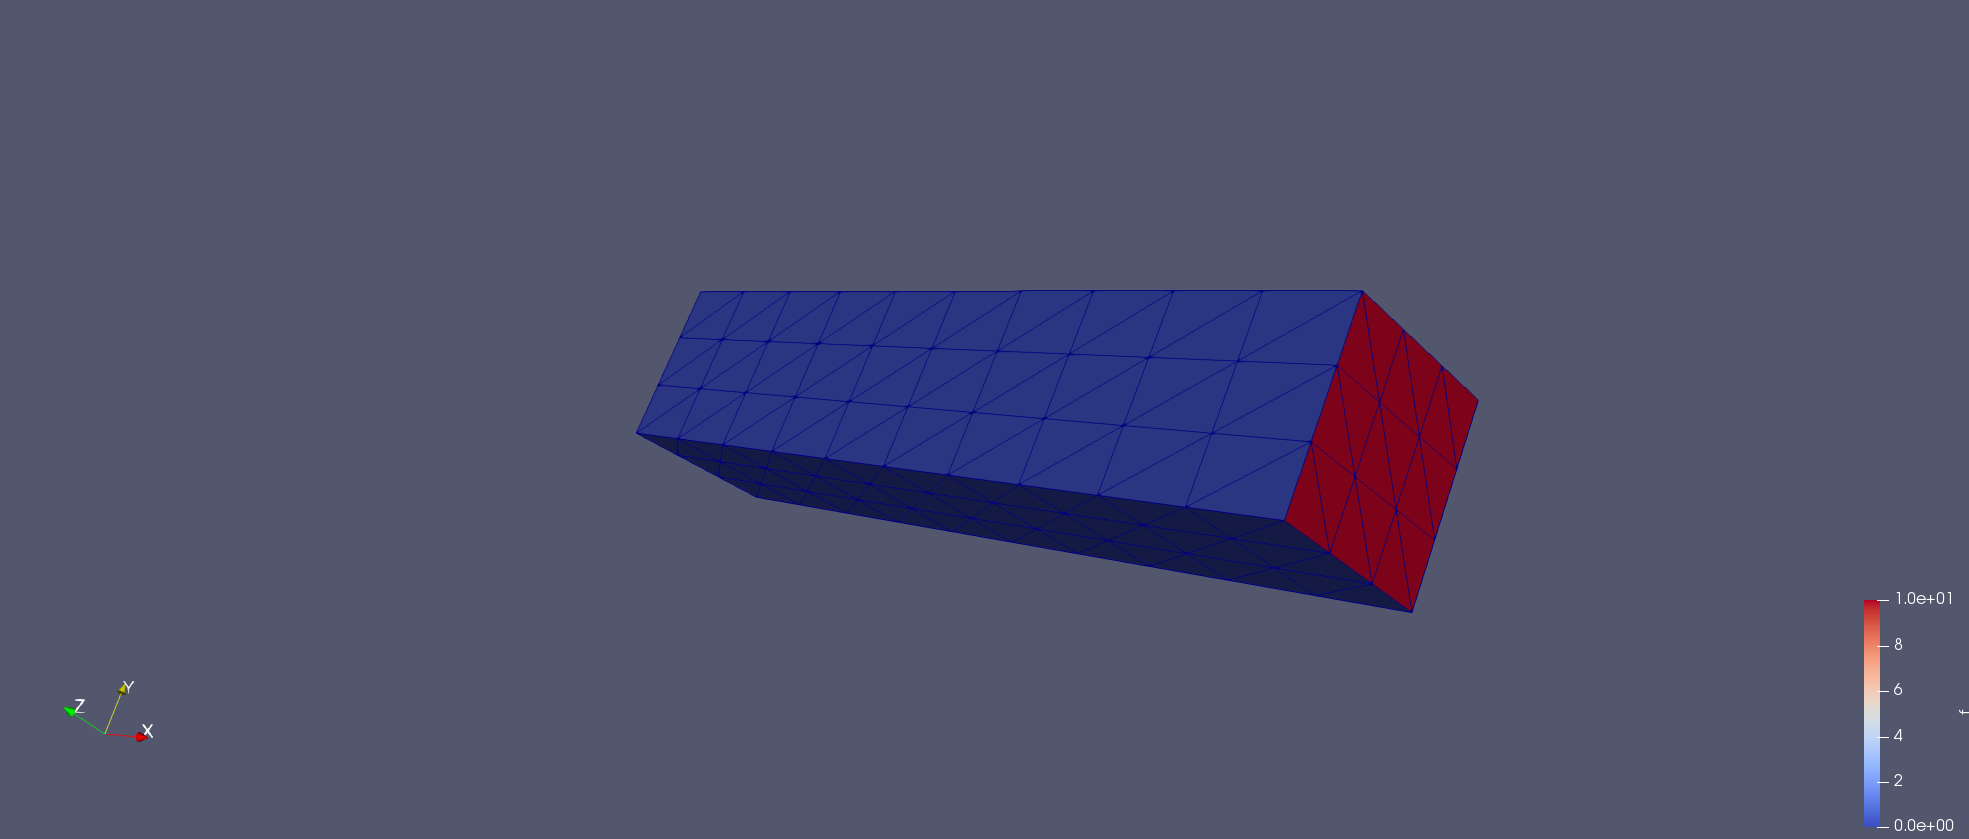
\includegraphics[width=.9\textwidth]{Right_End}
\end{figure}
\begin{itemize}
\vfill
		\item{So we can be sure that boundaries are set up right. The main change I made in the code is:}
				\begin{lstlisting}[language=Python, basicstyle=\ttfamily\small,  keywordstyle=\color{blue}]
sub_domains = FacetFunction("size_t", mesh) 
\end{lstlisting}
\vfill
		\item{Earlier I was using $MeshFunction$ which was wrong}	
\end{itemize}
\end{frame}

 \begin{frame}
\frametitle{Next step: Visualize the load}
\begin{itemize}
		\vfill
		\item{We can now rule out that boundaries are not part of the problem}
		\vfill
		\item{The next thing is to check if the load is applied correctly on right end by visualizing them}
		\vfill
\end{itemize}
\end{frame}


\end{document}